\documentclass{standalone}
\usepackage{pgf, tikz}
\usetikzlibrary{arrows, automata}
\begin{document}
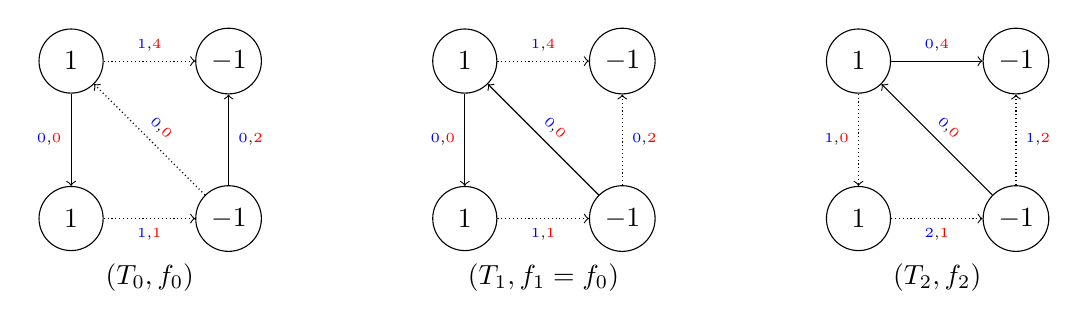
\begin{tikzpicture} [align=center]
\path (1,-0.75) node (t1) {$(T_0,f_0)$}
	  (6,-0.75) node (t2) {$(T_1,f_1=f_0)$}
	  (11,-0.75) node (t3) {$(T_2,f_2)$};

\path (0, 0) node[circle, draw, text width=0.44cm] (v0) {$1$}
	  (2, 0) node[circle, draw, text width=0.44cm] (v1) {$-1$}
	  (2, 2) node[circle, draw, text width=0.44cm] (v2) {$-1$}
	  (0, 2) node[circle, draw, text width=0.44cm] (v3) {$1$};
	  
\draw[densely dotted, ->] (v0) to node [below] {\tiny\textcolor{blue}{1},\textcolor{red}{$1$}} (v1);
\draw[->] (v1) to node [right] {\tiny\textcolor{blue}{0},\textcolor{red}{$2$}} (v2);
\draw[densely dotted, ->] (v3) to node [above] {\tiny\textcolor{blue}{1},\textcolor{red}{$4$}} (v2);
\draw[->] (v3) to node [left] {\tiny\textcolor{blue}{0},\textcolor{red}{$0$}} (v0);
\draw[densely dotted, ->] (v1) to node [sloped, anchor=center, above] {\tiny\textcolor{blue}{0},\textcolor{red}{$0$}} (v3);

\path (5, 0) node[circle, draw, text width=0.44cm] (v4) {$1$}
	  (7, 0) node[circle, draw, text width=0.44cm] (v5) {$-1$}
	  (7, 2) node[circle, draw, text width=0.44cm] (v6) {$-1$}
	  (5, 2) node[circle, draw, text width=0.44cm] (v7) {$1$};

\draw[densely dotted, ->] (v4) to node [below] {\tiny\textcolor{blue}{1},\textcolor{red}{$1$}} (v5);
\draw[densely dotted, ->] (v5) to node [right] {\tiny\textcolor{blue}{0},\textcolor{red}{$2$}} (v6);
\draw[densely dotted, ->] (v7) to node [above] {\tiny\textcolor{blue}{1},\textcolor{red}{$4$}} (v6);
\draw[->] (v7) to node [left] {\tiny\textcolor{blue}{0},\textcolor{red}{$0$}} (v4);
\draw[->] (v5) to node [sloped, anchor=center, above] {\tiny\textcolor{blue}{0},\textcolor{red}{$0$}} (v7);

\path (10, 0) node[circle, draw, text width=0.44cm] (v8) {$1$}
	  (12, 0) node[circle, draw, text width=0.44cm] (v9) {$-1$}
	  (12, 2) node[circle, draw, text width=0.44cm] (v10) {$-1$}
	  (10, 2) node[circle, draw, text width=0.44cm] (v11) {$1$};

\draw[densely dotted, ->] (v8) to node [below] {\tiny\textcolor{blue}{2},\textcolor{red}{$1$}} (v9);
\draw[densely dotted, ->] (v9) to node [right] {\tiny\textcolor{blue}{1},\textcolor{red}{$2$}} (v10);
\draw[->] (v11) to node [above] {\tiny\textcolor{blue}{0},\textcolor{red}{$4$}} (v10);
\draw[densely dotted, ->] (v11) to node [left] {\tiny\textcolor{blue}{1},\textcolor{red}{$0$}} (v8);
\draw[->] (v9) to node [sloped, anchor=center, above] {\tiny\textcolor{blue}{0},\textcolor{red}{$0$}} (v11);
\end{tikzpicture}
\end{document}